\documentclass{article}

%%%%%%%%%%%%%%%%%%%%%%%%%%%%%%%%%%%%%%%%%%%%%%%%
% This seciont would include all the required
% packages.
%%%%%%%%%%%%%%%%%%%%%%%%%%%%%%%%%%%%%%%%%%%%%%%%

% table of contents are in different lines.
\usepackage[utf8]{inputenc}

% for table's toprule and bottomrule
\usepackage{booktabs}

% code listing
\usepackage{tcolorbox}
\usepackage{listings}
\lstdefinestyle{mystyle}{
	backgroundcolor=\color{backcolour},   
	commentstyle=\color{codegreen},
	keywordstyle=\color{magenta},
	numberstyle=\tiny\color{codegray},
	stringstyle=\color{codepurple},
	basicstyle=\ttfamily\footnotesize,
	breakatwhitespace=false,         
	breaklines=true,                 
	captionpos=b,                    
	keepspaces=true,                 
	numbers=left,                    
	numbersep=5pt,                  
	showspaces=false,                
	showstringspaces=false,
	showtabs=false,                  
	tabsize=2
}
\lstset{style=mystyle}

% page dimensions
\usepackage{geometry}
\geometry{
	a4paper,
	total={170mm,257mm},
	left=20mm,
	top=20mm,
}

% captioned images or figures in LaTeX.
\usepackage{float}

% for referencing
\usepackage[%  
colorlinks=true,
pdfborder={0 0 0},
linkcolor=red
]{hyperref}

% to make caption bold.
% https://tex.stackexchange.com/a/32463/277097
\usepackage[labelfont=bf]{caption}

% colorbox
% https://texdoc.org/serve/tcolorbox.pdf/0
\usepackage{tcolorbox}

% citations
\usepackage{cite}

%%%%%%%%%%%%%%%%%%%%%%%%%%%%%%%%%%%%%%%%%%%%%%%%
% package end.
%%%%%%%%%%%%%%%%%%%%%%%%%%%%%%%%%%%%%%%%%%%%%%%%

\title{
	Masterarbeit \\
	Robust Registration to a template brain  \\
	for the Drosophila larva \large }

\author{Harsha Yogeshappa}

% define RWTH Color
% https://www.color-hex.com/color-palette/33602
\definecolor{rwth-blue-1}{rgb}{0.00, 0.33, 0.62}
\definecolor{rwth-blue-2}{rgb}{0.25, 0.50, 0.71}
\definecolor{rwth-blue-3}{rgb}{0.55, 0.72, 0.89}
\definecolor{rwth-blue-4}{rgb}{0.78, 0.87, 0.95}
\definecolor{rwth-blue-5}{rgb}{0.90, 0.94, 0.98}

\begin{document}
	\maketitle
	\newpage
	
	\hypersetup{linkcolor=rwth-blue-1}
	\tableofcontents
	\newpage
	\section{Introduction}
	In the field of medical imaging, image registration is an important application. Image registration involves two images in which one image is spatially transformed to align with the other image. This spatial alignment is necessary when comparing and examining the corresponding and/or complementary information. Figure \ref{fig:Registraion} shows one such registration example. \newline
		
	% https://tex.stackexchange.com/a/8633/277097
	\begin{figure}[H]
		\centering
		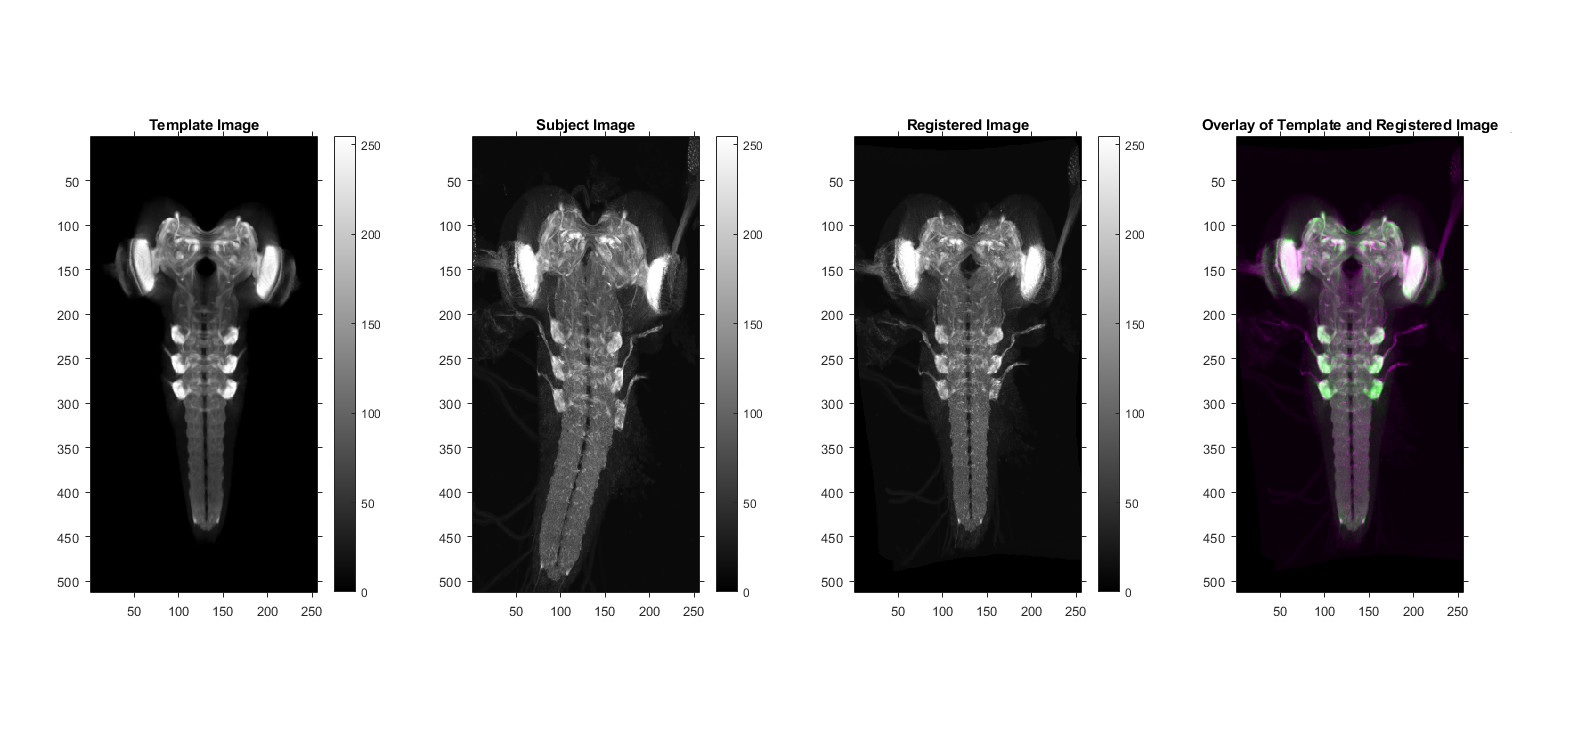
\includegraphics[width=\linewidth]{resources/introduction_fig_1.jpg}
		\caption{An image registration example: The subject image is registered against the target image, and the result is the registered image.}
		\label{fig:Registraion}
	\end{figure}

	The registered image is the same subject image, which is now displayed in the coordinate system of the target image. The last column is an overlay of the registered and the target image, which is a composite RGB image and the subject and the target images are overlaid in different color bands. The green areas correspond to the areas of the target image, while the magenta areas represent the areas of the registered image. In regions with perfect overlap, i.e. perfect registration, the regions are displayed in grayscale (or original intensity). This provides us with a perfect tool to visually check the registration discrepancies. \newline
			
	Whether in research laboratories where organisms are studied by biologists or in clinical applications, image registration is one of the most important steps in planning and monitoring changes over time. Therefore, it is important to make the image registration process robust and real time. \newline
	
	Registration of an image can be done in two ways - non-learning style or learning style. However, the non-learning style of registration presents a problem where the same registration errors are repeated each time registration is performed between the same image pair, and also registration must start over each time a new image pair must be registered.\newline
	
	In this work, image registration is made more robust and real-time by using deep learning techniques. It also offers the possibility of incorporating auxiliary information in the form of landmarks, segmentations or the like into the training to steer the network in the right learning direction.

	\subsection{Motivation}
	The thesis is an extension of the work done in the \emph{larvalign} paper \cite{Mu_2018}. \emph{larvalign} is both a standard 3D volume template constructed using \emph{PB Method} (van Hecke et al. 2008 \cite{Hecke_2008}, van van Pelt 2013 \cite{Pelt_2013}) and a registration method to register any given 3D volume to another 3D volume or to the \emph{larvalign}. \newline
	
	Though the \emph{larvalign} showed promising results, it however, on few images, failed to perform successful registration especially at the lower tip of the Ventral Nerve Cord (VNC) which can be seen in the figure \ref{fig:Registraion_Failure}. \newline
		
	Like figure \ref{fig:Registraion}, figure \ref{fig:Registraion_Failure} is also an example of \emph{larvalign} registration. The magenta structure at the lower tip of the ventral nerve cord in the overlay is a registration error. \newline
	
	\begin{tcolorbox}[colback=rwth-blue-5,colframe=rwth-blue-1,title=\textbf{Note}]
		In the field of image registration, the target image against which the registration is performed is referred to as "fixed" image, the subject image which needs to be registered is referred to as "moving" image, and finally, the registered image itself is referred to as "moved" image.
		\tcblower
		Thus, from now on, we will stick to this nomenclature throughout the thesis.
	\end{tcolorbox}
	
	\begin{figure}[H]
		\centering
		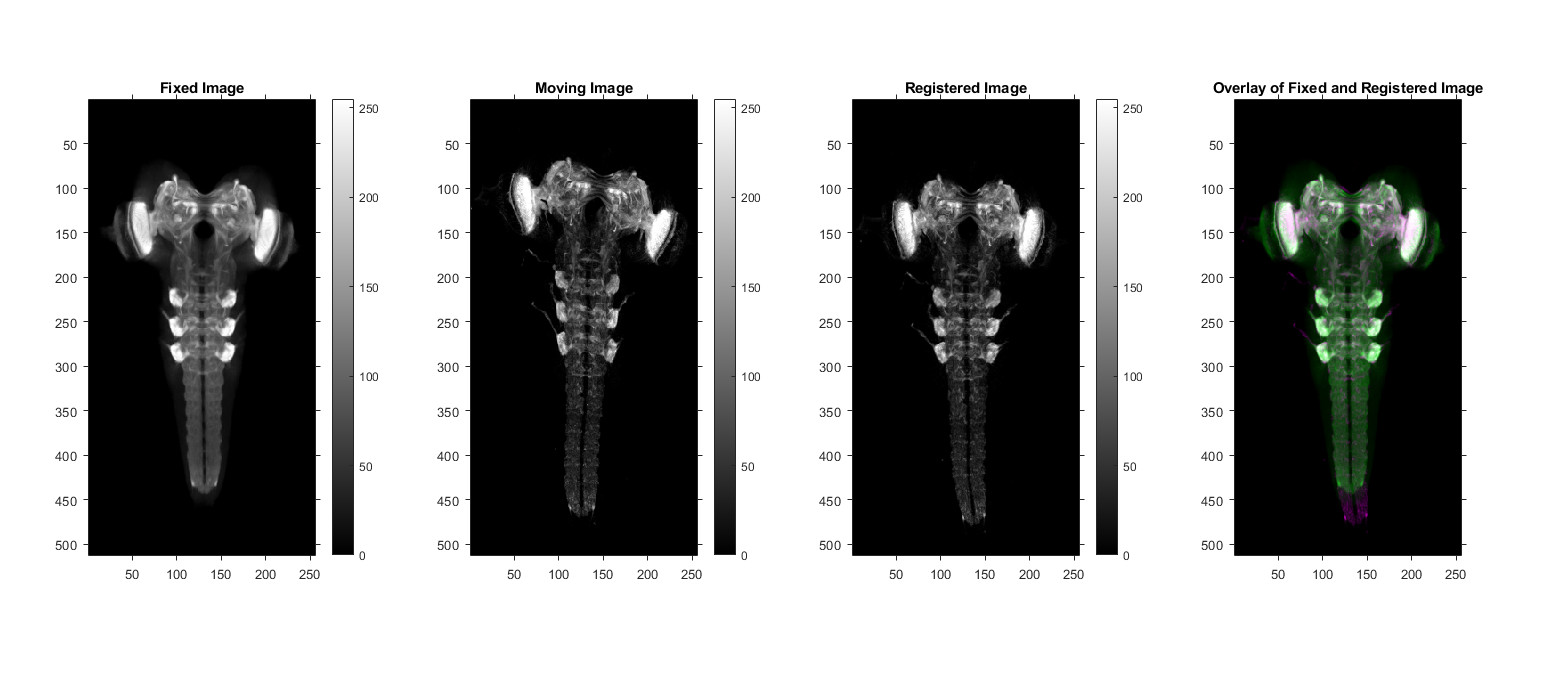
\includegraphics[width=\linewidth]{resources/motivation_fig_1.jpg}
		\caption{Registration failure example of \emph{larvalign} at lower tip of Ventral Nerve Cord.}
		\label{fig:Registraion_Failure}
	\end{figure}
	
	\emph{larvalign} is by definition a non-learning way of performing registration, i.e. it performs registration between new image pairs from the scratch and repeats the same errors each time it performs registration. We are attempting to solve these problems by moving from a non-learning type of registration to a learning type, in the hope that the model will learn to solve these registration problems through experience. Since deep learning techniques allow the model to learn a function that can quickly compute the deformation field between pairs of images, we also hope that the time required to perform registration should be much less time consuming than existing non-learning methods \cite{Voxelmorph} \cite{deVos_2018} \cite{Wu_2016} \cite{Yang_2017} \cite{Hessam_2017}.
	
	\subsection{Model organism - Drosophila larva}
	
	In this work, as in \emph{larvalign} \cite{Mu_2018}, the 3D scans of the central nervous system of Drosophila melanogaster at its larval stage are used. Drosophila melanogaster, commonly known as the fruit fly, has been used in scientific research and neuroscience for about a century, according to the University of Michigan Museum of Zoology. One of the reasons Drosophila is such an ideal research subject is that it has a short life span and can reproduce very quickly. It matures into an adult in 7 days, and a female can produce 100 eggs a day; the female fruit fly lays about 750-1,500 eggs in her lifetime. This allows researchers to study many generations in a short period of time. \newline
	
	Drosophila develops holometabolically, meaning it has three distinct stages of its life cycle after embryonic development: Larva, pupa and finally the adult. The larval stage itself has 3 sub-stages, referred to as 3 instars, lasting a total of about 4-5 days. During the larval stage, most cell types are already differentiated and functional \cite{cherry_biotech}. The central nervous system consists of only 10000 neurons \cite{Nassif_2003} compared to more than 250000 in adult flies and more than 86 billion neurons in humans, which is a simpler model. It is found that despite the simplicity in larval brain, it shares many structural features of the adult \cite{Mu_2018}. \newline
	
	Because of the rich history of Drosophila research, there are many systems that allow for easy research, such as many systems for manipulating gene expression and visualizing changes \cite{kalderon_lab}. In addition, an estimated 60\% of Drosophila genes have homologs in humans, making it a perfectly suitable tool not only to understand the molecular basis of human diseases, but also to study the function of these molecules in healthy organisms \cite{genome}.
	
	\begin{figure}[H]
		\centering
		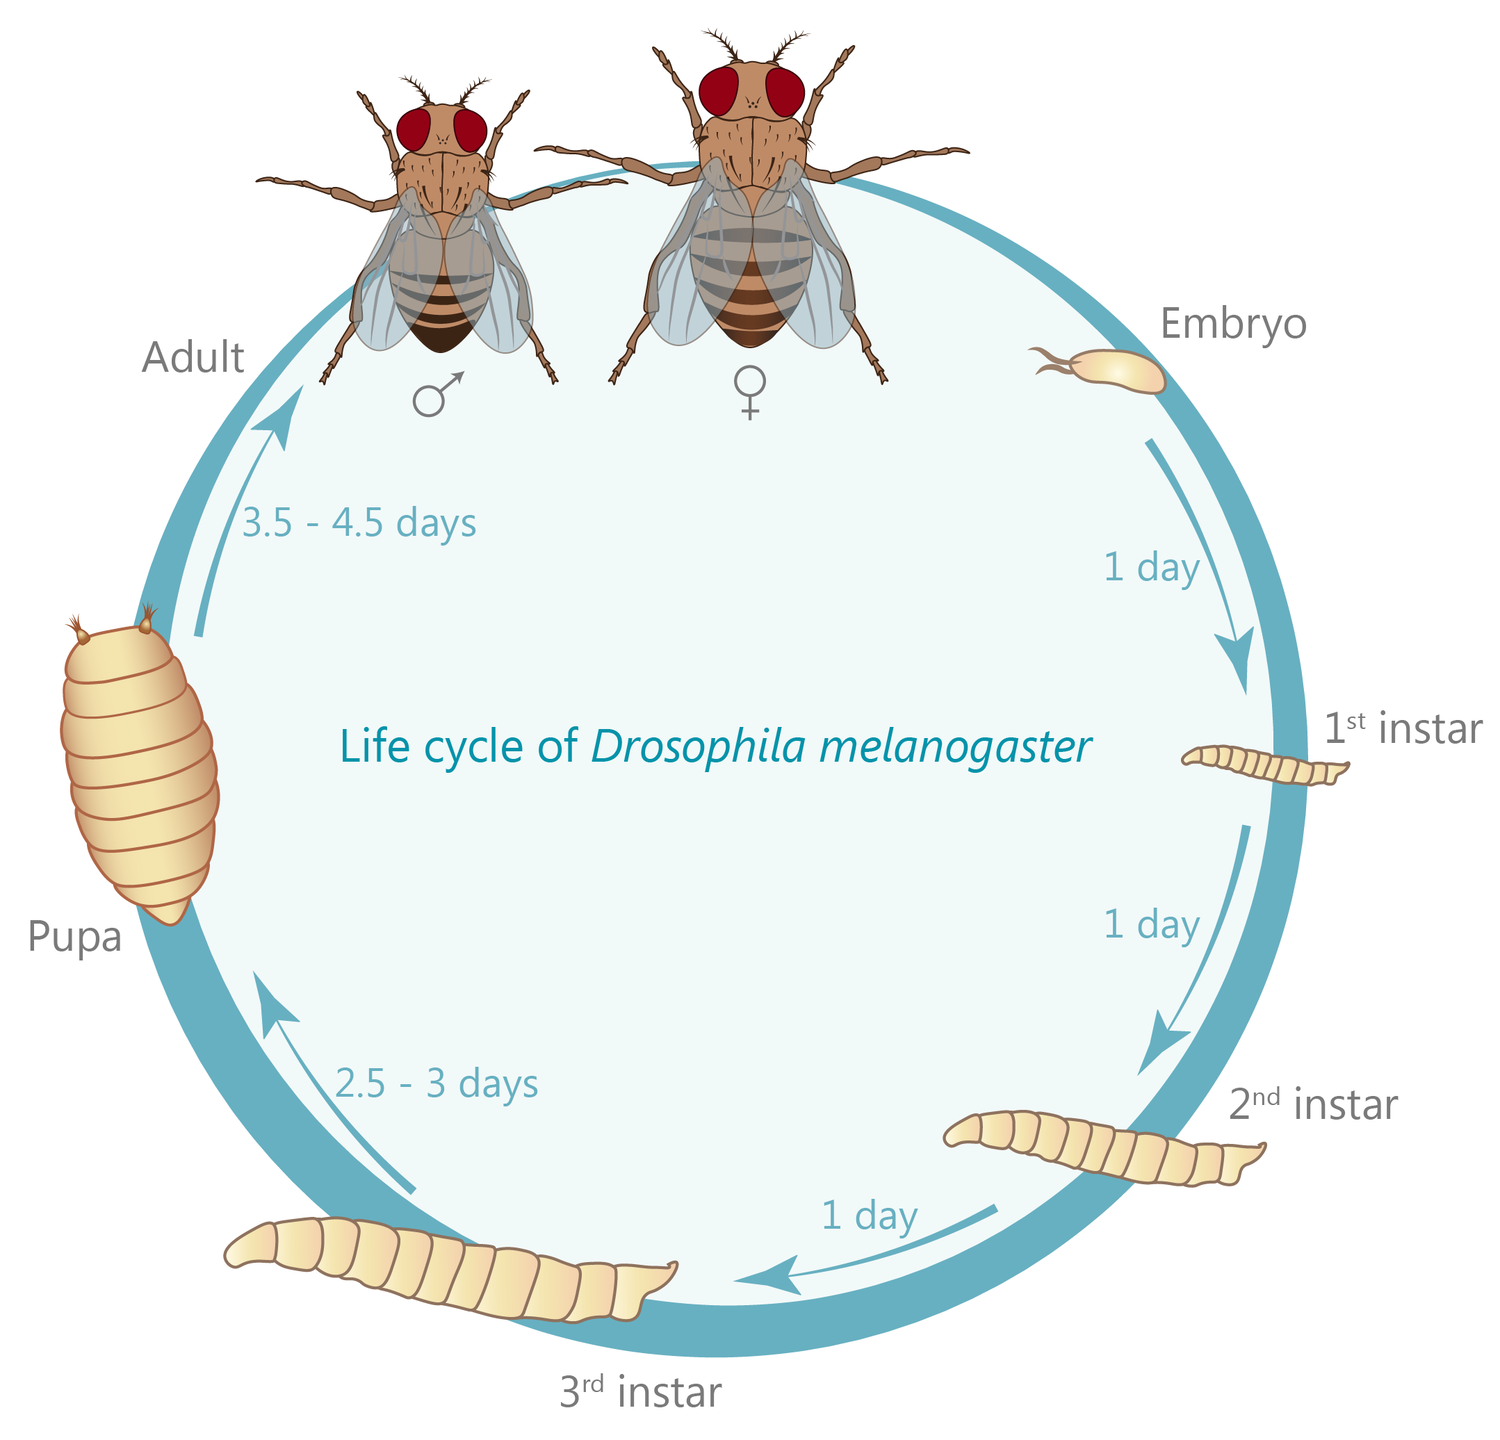
\includegraphics[width=0.7\columnwidth]{resources/model_organism_fig_1.png}
		\caption{Life cycle of Drosophila melanogaster. \cite{walter}}
		\label{fig:Life_cycle_of_fruit_fly}
	\end{figure}
	
	Detailed study of the brain of any animal can reveal the general principles of function of all brains \cite{Scheffer_2020}. The study of adult flies has also led to important discoveries in basic biological processes such as aging, circadian clocks, and behavioral studies \cite{cherry_biotech}. Fruit flies support a range of complex behaviors - active flight maneuvers, learning, responses to sensory stimuli such as odors and light. A fruit fly can complete a 120-degree turn in just 18 wing beats, and each wing beat takes about 4 milliseconds \cite{wired}. Considering that each blink of a human's eye takes between 0.1 and 0.4 seconds, the fruit fly would complete a full 180-degree turn with one blink.  

	\subsection{Organization}
	This section provides a brief description of the rest of the chapters in the report.
	
	\textbf{Chapter 2} A discussion on the \emph{larvalign} paper and the related works in deep learning based deformable image registrations is provided. Finally, the base method used in the thesis work is presented. 
	
	\textbf{Chapter 3} The details of the dataset used and implementation is mentioned. A novel landmark-based auxiliary information is proposed and implemented.
	
	\textbf{Chapter 4} This entails the results and the metrics used for evaluation, both qualitative and quantitative, are mentioned and discussed.
	
	\textbf{Chapter 5} This includes the analysis and interpretation of the findings.
	
	\textbf{Chapter 6} This chapter provides the conclusion and the future work.
	
	\section{Related Works}
	
	The registration can be done in two styles - non-learning style and learning style.	One such non-learning style of doing is using \emph{elastix} Image Registration Toolkit which is a parametric method and uses an iterative approach to find the optimal solution. The success or the failure of such parametric methods depend on the choice of the parameters and the optimal combination of these parameters\footnote{There are several such parameters available at our disposal.}. Also, the parameters are in a high dimensional space and the iterative approach makes the whole process time consuming. This makes the method highly data dependent, i.e., parameters optimized for one data set may or may not work for another data set. It would be desirable to develop a closed-form solution that works for all data. However, the high dimensionality of the parameter space makes it difficult to find a closed-form solution \cite{Fu_2020}. \newline
	
	
	\section{Materials and Methods}
	
	\section{Results}
	\subsection{Metrics}
	\subsection{Quality Assessment}
	\subsubsection{Qualitative Assessment}
	\subsubsection{Quantitative Assessment}
	
	\section{Discussion}
	
	\begin{tabular}{lr}
		\toprule
		landmark\_name                               &   error \\
		\midrule
		a6 left nerve entry                         &       0 \\
		a6 right nerve entry                        &       0 \\
		a7 left nerve entry                         &       0 \\
		a7 right nerve entry                        &       0 \\
		a8 left nerve entry                         &       0 \\
		a8 right nerve entry                        &       0 \\
		anterior upper commisure                    &       0 \\
		center sez neuropil fusion                  &       0 \\
		end of ventral nerve cord                   &       0 \\
		left antennal nerve                         &       0 \\
		left anterior lon nerve                     &       0 \\
		left basal brain neuropil border posterior  &       0 \\
		left mb vertical medial lobe connection     &       0 \\
		left thoracic nerve entry t1                &       0 \\
		left thoracic nerve entry t2                &       0 \\
		left thoracic nerve entry t3                &       0 \\
		left tip of vertical lobe                   &       0 \\
		left upper most nerve entry                 &       0 \\
		left upper peduncle                         &       0 \\
		posterior upper commisure                   &       0 \\
		right antennal nerve                        &       0 \\
		right anterior lon nerve                    &       0 \\
		right basal brain neruopil border posterior &       0 \\
		right mb vertical medial lobe connection    &       0 \\
		right thoracic nerve entry t1               &       0 \\
		right thoracic nerve entry t2               &       0 \\
		right thoracic nerve entry t3               &       0 \\
		right tip of vertical lobe                  &       0 \\
		right upper most nerve entry                &       0 \\
		right upper peduncle                        &       0 \\
		\bottomrule
	\end{tabular}
	
	\section{Conclusion}
	
	% bibiliography
	\newpage
	\bibliographystyle{ieeetr}
	\bibliography{./references}
\end{document}